\documentclass[conference]{IEEEtran}
\usepackage[spanish]{babel}
\usepackage[latin1]{inputenc}
\usepackage{blindtext, graphicx}
\usepackage{subfigure}
\usepackage{mdwmath}
\usepackage{mdwtab}
\usepackage{subfig}
\usepackage{amsmath}

\begin{document}
\title{ Implementaci\'on de la transformada Hough para encontrar el punto de fuga en una imagen }
\author{\IEEEauthorblockN{Walter Alejandro Moreno Ram\'irez}
\IEEEauthorblockA{Departamento de Estudios Multidisciplinarios\\
Universidad de Guanajuato\\
Yuriria, Guanajuato\\
Correo: wa.morenoramirez@ugto.mx}}

\maketitle
\renewcommand\abstractname{Abstract}
\begin{abstract}
This article describes how to implement the Hough transform, which are the most important applications and their advantages and disadvantages. Also, it describes how to find the vanishing point in an image. \\\\
\end{abstract}

\begin{IEEEkeywords}
Pixel, p\'ixeles, convoluci\'on, canny, smoothing, suavizado, gradiente, segmentaci\'on ,primera derivada, funci\'on, C++, OpenCV, ventana, m\'ascara, vecindario.
\end{IEEEkeywords}

\IEEEpeerreviewmaketitle
\section{Introducci\'on}
La transformada Hough es una t\'ecnica para la detecci\'on de figuras en im\'agenes digitales. Las figuras que se pueden detectar son c\'irculos, cuadrados, elipses y lineas rectas o curvas. Una caracter\'istica importante que debe cumplir toda figura para poder ser detectada por esta t\'ecnica es que puedan ser expresadas matem\'aticamente mediante una ecuaci\'on. \\\\
La transformada de Hough fue propuesta y patentada Paul Hough en 1962, pero fue hasta 1972 que Duda R. O. y P.E. Hart crearon la transformada de Hough tal como se conoce y utiliza actualmente quienes la llamaron ``Use of the Hough Transformation to Detect Lines and Curves in Pictures''. Pero fue Dana H. Ballard quien la populariz\'o en la comunidad de visi\'on por computadora publicando un art\'iculo en 1981, llamado ``Generalizing the Hough Transform to Detect Arbitrary Shapes''.\\

Para poder llevar a cabo la detecci\'on de lineas y curvas utilizando la transformada de Hough, como paso anterior es necesario obtener los bordes de los objetos, que es el resultado de la implementaci\'on del algoritmo de Canny para la detecci\'on de bordes o aplicando cualquier gradiente para obtener bordes como pueden ser: Prewitt, Sobel, Roberts, etc. \\
Esto es necesario para tener una menor cantidad de elementos no requeridos y que pudieran afectar en la detecci\'on de lineas o curvas y, tambi\'en pudieran provocar un tiempo de ejecuci\'on muy alto.

Para esta pr\'actica, se utiliz\'o la transformada de Hough para encontrar el punto de fuga de una imagen. Un elemento importante en una imagen digital es el punto de fuga ya que nos ayuda a dar profundidad a la imagen a trav\'es de lineas reales o imaginarias que convergen en un punto infinito. Si observamos una carretera o unas v\'ias de tren, a medida que se alejan parece acercarse hasta converger en un mismo punto, es ese preciso momento donde observamos como las l\'ineas parecen curzarse es lo que se llama punto de fuga en una imagen y utilizando la transformada de Hough lo obtendremos.\\

\section{Metodolog\'ia}
El espacio de una imagen digital a cada pixel le corresponde una coordenada de la forma $(x,y)$, semejante al sistema de coordenadas rectangular o cartesiano. Esto nos facilita la detecci\'on de figuras y, en este caso, el objetvio es detectar las rectas presentes en una imagen. Para ello, la ecuaci\'on de la recta, que se muestra en la Ecuaci\'on (1), servir\'a para cumplir este cometido.

\begin{equation}
	y = m*x + b
\end{equation}

Y se puede graficar para cada par ordenado $(x,y)$ en la imagen. La transformada Hough se basa en considerar las caracter\'isticas de una recta en t\'ermino de sus par\'ametros $(m,b)$, y no como sus puntos de la imagen. Basandose en lo anterior, una recta que tiene la forma (1), puede representarse en el espacio param\'etrico como un punto. Sin embargo, cuando se tienen rectas verticales, los par\'ametros de la recta se indefinen. Para solucionar esto, se utilizan los par\'ametros que describen una recta en coordenadas polares, denotado por $(\rho , \theta )$.\\
El par\'ametro $\rho$ representa la distancia del origen de coordenadas y el punto $(x,y)$ y $\theta$ es el \'angulo del vector director de la recta perpendicular a la recta original y que pasa por el origen de coordenadas.\\
Utilizando esta parametrizaci\'on, la ecuaci\'on de la recta, mostrada en la Ecuaci\'on (1), se puede escribir como se muestra en la Ecuaci\'on (2).

\begin{equation}
	\rho = x\cos(\theta) + y\sin(\theta)
\end{equation}

Entonces, es posible asociar a cada rectar un par $(\rho,\theta)$ que es \'unico si $\theta \epsilon [0,\pi)$.\\
Sin embargo, por un s\'olo punto con coordenadas $(x,y)$ pasan un n\'umero infinito de rectas. Para poder discretizar este n\'umero de rectas en coordenadas $(\rho,\theta)$, lo mejor es considerar el intervalo $[0,\pi)$, lo que nos da como resultado una curva sinusoidal en el espacio $\rho-\theta$ para cada familia de rectas que pasan por un punto $(x,y)$. Entonces para cada punto en el plano cartesiano, tendremos una curva sinusoidal en el plano polar, con la posbilidad de que varias curvas sinusoidales se crucen en un mismo punto, indicando que son parte de una recta en el plano cartesiano.\\
Con esto logramos trasladar el problema de encontrar una secuencia de puntos o p\'ixeles que nos indiquen una recta a buscar un n\'umeros de intersecciones de varias curvas sinusoidales.\\\\
El valor m\'aximo de intersecciones entre curvas no representar\'a la recta dominante de la imagen y dicho valor puede servir como par\'ametro para encontrar las dem\'as rectas.\\

Se sigue el pseudoc\'odigo de la Figura 1. para poder realizar la conversi\'on de espacio $(x,y)$ a $(\rho,\theta)$.

\begin{figure}[h]
	\setlength{\unitlength}{0.105in}
	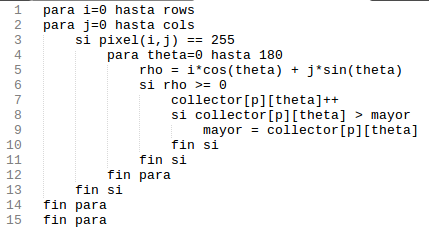
\includegraphics[scale=0.50]{./images/pseudo.png}
	\caption{ Pseudoc\'odigo para obtener las curvas sinusoidales para cada punto $(x,y)$ y el valor m\'aximo correspondiente 
			  a la recta dominante. }
\end{figure}

Se recorre la imagen de entrada completamente lo que permite poder obtener cada pixel para analizarlo, si dicho pixel es un borde, se procede a calcular una $\rho$ por cada $\theta$ que est\'a dentro del intervalo $[0,\pi)$, con cada par ordenado se incrementa en uno el acumulador, lo que nos dar\'a una curva sinusoidal como salida, ya que el acumulador puede mostrase como una imagen de salida pero se mostrar\'a en la secci\'on de resultados m\'as adelante.\\

Una vez se obtuvo la recta dominante, una manera para obtener otras rectas de la imagen es umbralizar el acumulador utilizando un porcentaje del valor de la recta dominante que en el pseudoc\'odigo se nombra como ``mayor'' o utilizando un valor arbitrario, como se muestra en la Figura 2.

\begin{figure}[h]
	\setlength{\unitlength}{0.105in}
	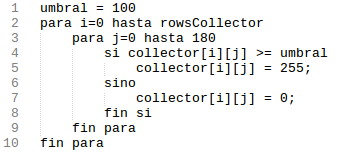
\includegraphics[scale=0.50]{./images/pseudo2.png}
	\caption{ Pseudoc\'odigo para umbralizar el acumulador y obtener las rectas dominantes de la imagen de entrada. }
\end{figure}

De esta manera, todos los valores que sean mayores o iguales al umbral ser\'an las rectas que se mostrar\'an al final, los que no cumplan la condici\'on se mandan a cero directamente.\\

Hasta el momento se tiene un acumulador s\'olo con los puntos $(\rho,\theta)$ pertenecientes a las rectas demoninanste, el siguiente procedimiento es volver del espacio polar al espacio cartesiano, para ello es necesario despejar la variable $y$ de la Ecuaci\'on (2), este resultado se muestra en la Ecuaci\'on (3).

\begin{equation}
	y = \frac{\rho - x\cos(\theta)}{\sin(\theta)}
\end{equation}

Y, de acuerdo al pseudoc\'odigo de la Figura 3, se recorre todo el acumulador buscando los valores que sean iguales a 255, lo que indica que son m\'aximos y rectas dominantes.

\begin{figure}[h]
	\setlength{\unitlength}{0.105in}
	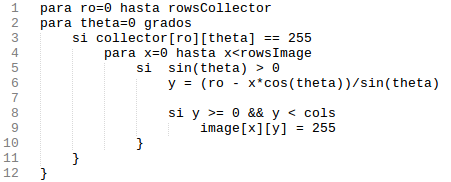
\includegraphics[scale=0.50]{./images/pseudo3.png}
	\caption{ Pseudoc\'odigo para pasar de coordenadas polares a coordenadas cartesianas con los puntos m\'aximos. }
\end{figure}

Al momento de despejar $y$ de (2), se obtiene la ecuaci\'on de la recta, por lo tanto tendremos que iterar con una sola variable, tal como se hizo para encontrar las curvas sinusoidales, para poder encontrar el valor de la variable dependiente.\\\\ Algo que se debe verificar es que la evaluaci\'on de $\sin(\theta)$ no sea cero, ya que se encuentra en el denominador y puede dar un resultado no definido para $\rho$, esto se arregla incluyendo una condici\'on para que s\'olo acepte valores positivos y, de igual manera, cuidando que los valores de $\rho$ no se salgan de las dimensiones de la imagen. Si ambas condiciones se cumplen, la imagen en el punto $(x,y)$ recien calculado, se pone en alto o 255, lo que nos da como resultado una recta para cada punto $(\rho,\theta)$.\\\\

\section{Resultados}
Para la presente pr\'actica se utiliz\'o una fotograf\'ia de un pasillo del Departamento de Estudios Multisciplinarios, mas especificamente el pasillo que conduce al laboratorio. Dicha foto se muestra en la Figura 4.

\begin{figure}[h]
	\setlength{\unitlength}{0.105in}
	\centering
	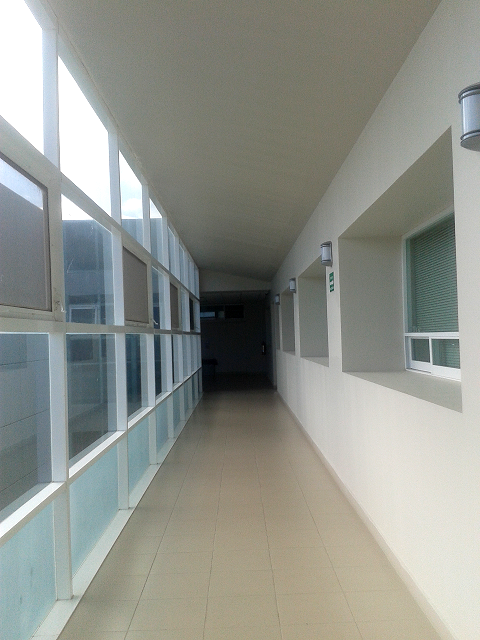
\includegraphics[scale=0.25]{./images/dem1.png}
	\caption{ Imagen de prueba para probar la implementaci\'on de la transformada de Hough. }
\end{figure}

\newpage
Debido a que, para aplicar la transformada de Hough, es necesario trabajar con los bordes de una imagen, esto se obtiene de la implementaci\'on del algoritmo de Canny y se muestra en la Figura 5.

\begin{figure}[h]
	\setlength{\unitlength}{0.105in}
	\centering
	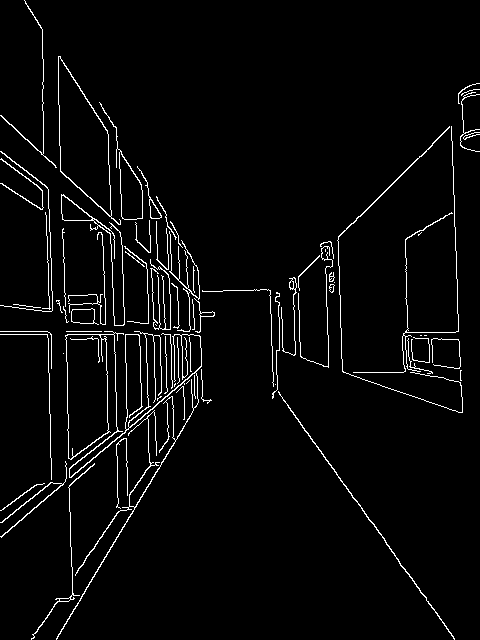
\includegraphics[scale=0.35]{./images/dem.png}
	\caption{ Bordes de la imagen de prueba. }
\end{figure}

Se puede visualizar el acumulador que contiene todas las curvas sinusoidales correspondientes a cada punto de la imagen con los bordes, esto se muestra en la Figura 6. Las imagenes resultantes de los acumuladores son sorprendetes y muy llamativas.

\begin{figure}[h]
	\setlength{\unitlength}{0.105in}
	\centering
	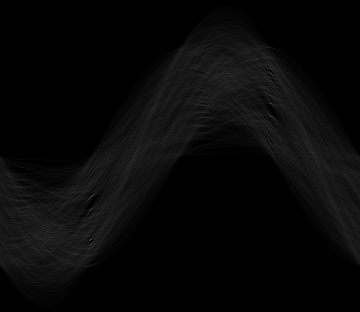
\includegraphics[scale=0.60]{./images/collector.png}
	\caption{ Acumulador correspondiente a los bordes de la imagen de prueba. }
\end{figure}

\newpage
La imagen obtenida aplicando la transformada de Hough a la imagen con los bordes se mustra en la Figura 7. Se utiliz\'o un umbral de 100 para encontrar las lineas rectas dominantes.

\begin{figure}[h]
	\setlength{\unitlength}{0.105in}
	\centering
	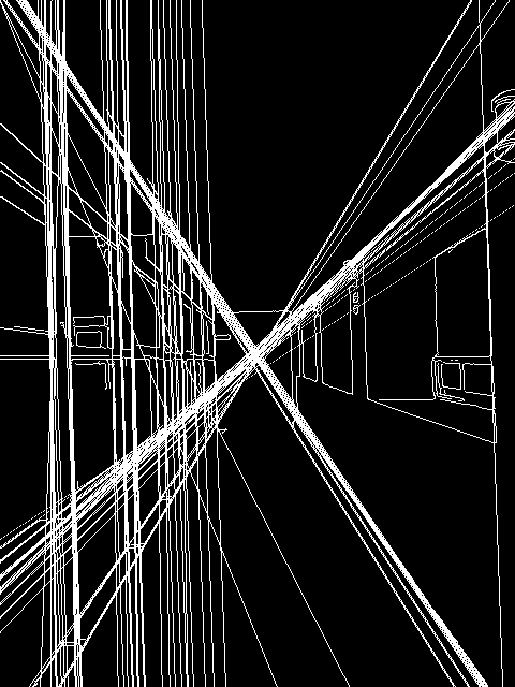
\includegraphics[scale=0.35]{./images/lineas.png}
	\caption{ Lineas principales detectadas con la transformada Hough y punto de fuga. }
\end{figure}

De la Figura 7. podemos apreciar como la mayor\'ia de lineas convergen hacia un punto central, lo que se conoce como punto de fuga de una imagen. \\

\section{Conclusiones}
La taransformada de Hough puede aplicarse para detectar m\'as figuras, no \'unicamente lineas, pero ya que se detectaron las lineas se pueden encontrar figuras que est\'en formadas por dichas lineas como pueden ser: cuadrados, tri\'angulos, trapecios, etc. Sin embargo, tambi\'en se pueden detectar curvas, elipses y c\'irculos, para ello es necesario utilizar sus respectivas ecuaciones.\\
Una aplicaci\'on simple que se le puede dar es detectar la orientaci\'on de una pieza u objeto dentro de una barra transportadora en una linea de production, para que un brazo rob\'otico pueda re-orientar su mano y poder tomar la pieza.


%$\begin{bmatrix}
% 1 & 1 & 1 & 1 \\
% 1 & 1 & 1 & 1 \\
% 1 & 1 & 1 & 1 \\
% 1 & 1 & 1 & 1 \\
%\end{bmatrix}$

%\begin{thebibliography}{1}
%    \bibitem{IEEEhowto:kopka}
%    H.~Kopka and P.~W. Daly, \emph{A Guide to \LaTeX}, 3rd~ed.\hskip 1em plus
%      0.5em minus 0.4em\relax Harlow, England: Addison-Wesley, 1999.
%\end{thebibliography}

\end{document}
